\documentclass[11pt,twoside,a4paper]{article}
\usepackage[T1]{fontenc}
\usepackage[utf8]{inputenc}
\usepackage[top=20mm, head=6mm, headsep=6mm, foot=6mm, bottom= 15mm, left=15mm, right=15mm]{geometry}
\usepackage{amsmath}
\usepackage{tikz}
\usetikzlibrary{automata,positioning}
\usepackage{calc} 
\usepackage{pythontex}
\newcommand{\mylabel}[1]{#1\hfill}
\renewenvironment{itemize}
  {\begin{list}{$\triangleright$}{%
   \setlength{\parskip}{0mm}
   \setlength{\topsep}{.4\baselineskip}
   \setlength{\rightmargin}{0mm}
   \setlength{\listparindent}{0mm}
   \setlength{\itemindent}{0mm}
   \setlength{\labelwidth}{2ex}
   \setlength{\itemsep}{.4\baselineskip}
   \setlength{\parsep}{0mm}
   \setlength{\partopsep}{0mm}
   \setlength{\labelsep}{1ex}
   \setlength{\leftmargin}{\labelwidth+\labelsep}
   \let\makelabel\mylabel}}{%
   \end{list}\vspace*{-1.3mm}}
\parindent0ex
\parskip2ex
\newcounter{quesito}
\newenvironment{question}{\bigskip\addtocounter{quesito}{1}\bigskip\bigskip\par\textbf{Quesito \thequesito.\kern1ex}}{\vspace{\parskip}}
\newenvironment{xquestion}{\bigskip\addtocounter{quesito}{1}\bigskip\bigskip\par\textbf{Quesito \thequesito.\kern1ex}}{\vspace{\parskip}}
\newenvironment{answer}{\par\textbf{Risposta\quad}}{\vspace{\parskip}}

\pagestyle{empty} 

\begin{document}
\colorbox{blue!10}{\begin{minipage}{\textwidth}
Domande  (qualcuna artificiale) per verificare la comprensione della definizione di distribuzione di probabilità,  valore atteso, e varianza per le v.a. discrete. Anche un esercizio sul teorema delle probabilità totali.
\end{minipage}}

\bigskip\bigskip


\begin{pycode}
import random
random.seed(258466445)
\end{pycode}

%1
\begin{question}
\def\Pr{{\rm Pr\,}}
\def\Ex{{\rm E\,}}
\def\Var{{\rm Var\,}}
\begin{pycode}
from sympy import Rational, latex
x = random.sample([1,2,3],2)
x1 = -x[0]
x2 = x[1]
x3 = x[0]
p1 = Rational(1,random.choice([2,3,4]))
p2 = Rational(1,random.choice([3,4]))
p3 = 1- p1 - p2
\end{pycode}
La v.a.\@ discreta $X$ ha distribuzione di probabilità 

\hfil$\displaystyle\Pr(X=\py{x1}) =\py{latex(p1)}$,\hfil  $\displaystyle\Pr(X=\py{x2}) =\py{latex(p2)}$,\hfil $\displaystyle\Pr(X=\py{x3}) =\py{latex(p3)}$. 

\begin{itemize}
\item[1.] Calcolare la distribuzione di probabilità di $X^2$
\item[2.] Calcolare $\Var(X)$. 
\end{itemize}

Esprimere i numeri razionali come frazioni.


\begin{answer}

{\color{blue}$\displaystyle\Pr(X^2=\py{x1**2})\ =\ \py{latex(p1+p3)}$ 
\ \ e \ \ 
$\displaystyle\Pr(X^2=\py{x2**2})\ =\ \py{latex(p2)}$\hfill Risposta 1} 

$\displaystyle\Ex(X) = \py{x1}\cdot\Pr(X=\py{x1})+\py{x2}\cdot\Pr(X=\py{x2})+\py{x3}\cdot\Pr(X=\py{x3})=\py{latex(x1*p1)} + \py{latex(x2*p2)} + \py{latex(x3*p3)}=\py{latex(x1*p1 + x2*p2 + x3*p3)}$

$\displaystyle\Ex(X^2) = \py{x1**2}\cdot\Pr(X^2=\py{x1**2})\ +\ \py{x2**2}\cdot\Pr(X^2=\py{x2**2})=\py{latex((x1**2)*(p1+p3))} + \py{latex((x2**2)*p2)} = \py{latex((x1**2)*(p1+p3)+ (x2**2)*p2)}$

$\displaystyle{\color{blue}\Var(X)}=\Ex(X^2)-\Ex(X)^2=\py{latex((x1**2)*(p1+p3)+ (x2**2)*p2)} - \py{latex((x1*p1 + x2*p2 + x3*p3)**2)}$ {\color{blue}$\ =\ \displaystyle\py{latex((x1**2)*(p1+p3)+ (x2**2)*p2 - (x1*p1 + x2*p2 + x3*p3)**2)} $\hfill Risposta 2} 
\end{answer}
\end{question}


%2
\begin{question}
\def\Pr{{\rm Pr\,}}
\def\Ex{{\rm E\,}}
\def\Var{{\rm Var\,}}
\begin{pycode}
from sympy import  Rational, latex
x = random.sample([1,2,3,4,5,6],2)
y = random.choice([2,3])
mu = x[0]
var = x[1]
\end{pycode}
La v.a.\@ discreta $X$ ha valore atteso $\Ex(X)=\py{mu}$ e varianza $\Var(X)=\py{var}$. Qual è il valore atteso di $X(X-\py{y})$?  
\begin{answer}

$\displaystyle{\color{blue}\Ex\big(X(X-\py{y})\big)}=\Ex(X^2)-\py{y}\cdot\Ex(X)=\Var(X)+\Ex(X)^2-\py{y}\cdot\Ex(X)${\color{blue}$\ =\ \displaystyle\py{var+mu**2-y*mu}$\hfill Risposta} 
\end{answer}
\end{question}


\clearpage
%3
\begin{question}
\def\Pr{{\rm Pr\,}}
\def\Ex{{\rm E\,}}
\def\Var{{\rm Var\,}}
\begin{pycode}
from sympy import  Rational, latex
x = random.sample([2,3,4,5],2)
x1 = x[0]
x2 = x[1]

p = random.sample([2,3,4,5],2)
d = random.choice(list(range(1,p[0])))
px = Rational(d,p[0])
d = random.choice(list(range(1,p[1])))
py = Rational(d,p[1])

\end{pycode}
Le v.a.\@ discrete $X$ e $Y$ sono indipendenti. La loro distribuzione di probabilità è data da 


\noindent\rlap{\kern15ex$\displaystyle\Pr(X=\py{x1}) =\py{latex(px)}$}\kern44ex   $\displaystyle\Pr(Y=1) =\py{latex(py)}$ 


\noindent\rlap{\kern15ex$\displaystyle\Pr(X=\py{x2}) =\py{latex(1-px)}$}\kern44ex $\displaystyle\Pr(Y=0) =\py{latex(1-py)}$

\begin{itemize}
\item[1.] Calcolare la distribuzione di probabilità di $X\cdot Y$
\item[2.] Calcolare $\Ex(X\cdot Y)$. 
\end{itemize}

Esprimere i numeri razionali come frazioni.
 
\begin{answer}

$\displaystyle\Pr(X\cdot Y=\py{x1})$ {\color{blue}$\displaystyle\ =\ \py{latex(px * py)}$}
\hfill 
$\displaystyle\Pr(X\cdot Y=\py{x2})$ {\color{blue}$\displaystyle\ =\ \py{latex((1-px) * py)}$}
\hfill 
$\displaystyle\Pr(X\cdot Y=0)$ {\color{blue}$\displaystyle\ =\ \py{latex(1-py)}$\hfill Risposta 1} 

$\displaystyle{\color{blue}\Ex(X\cdot Y)}\ =\ \py{x1}\cdot\Pr(X\cdot Y=\py{x1}) + \py{x2}\cdot\Pr(X\cdot Y=\py{x2})${\color{blue}$\ =\ \displaystyle\py{latex(x1 * px * py + x2 * (1-px) * py)}$\hfill Risposta 2} 

\end{answer}

\end{question}


%4
\begin{question}
\def\Pr{{\rm Pr\,}}
\def\Ex{{\rm E\,}}
\def\Var{{\rm Var\,}}
\begin{pycode}
from sympy import Rational, latex
a = random.choice( [1, 2, 3, 4] )

p = random.sample([2,3,4,5],2)
d = random.choice(list(range(1,p[0])))
px = Rational(d,p[0])
d = random.choice(list(range(1,p[1])))
py = Rational(d,p[1])
\end{pycode}
Le v.a.\@ discrete $X$ e $Y$ sono indipendenti. La loro distribuzione di probabilità è data da 


\noindent\rlap{\kern15ex$\displaystyle\Pr(X=\py{a})\phantom{-} =\py{latex(px)}$}\kern44ex   $\displaystyle\Pr(Y=\py{a})\phantom{-} =\py{latex(py)}$ 


\noindent\rlap{\kern15ex$\displaystyle\Pr(X=\py{-a}) =\py{latex(1-px)}$}\kern44ex $\displaystyle\Pr(Y=\py{-a}) =\py{latex(1-py)}$

\begin{itemize}
\item[1.] Calcolare la distribuzione di probabilità di $X + Y$
\item[2.] Calcolare $\Ex(X + Y)$. 
\end{itemize}

Esprimere i numeri razionali come frazioni.
 
\begin{answer}

{\color{blue}$\displaystyle\Pr(X + Y=\py{2*a})\ =\ \py{latex(px * py)}$
\hfill 
$\displaystyle\Pr(X + Y=\py{-2*a})\ =\ \py{latex((1-px) * (1-py)) }$
\hfill 
$\displaystyle\Pr(X + Y=0)\ =\ \py{latex(px+py-2*px*py)}$\hfill Risposta 1} 

$\displaystyle{\color{blue}\Ex(X + Y)}\ =\ \py{2*a}\cdot\Pr(X\cdot Y=\py{2*a}) \ - \py{2*a}\cdot\Pr(X\cdot Y=\py{-2*a})${\color{blue}$\ =\ \displaystyle\py{latex(2 * a * px * py - 2 * a * (1-px) *  (1-py))}$\hfill Risposta 2} 

\end{answer}
\end{question}



\clearpage
%5
\begin{question}
\def\Pr{{\rm Pr\,}}
\def\Ex{{\rm E\,}}
\def\Var{{\rm Var\,}}
\begin{pycode}
from sympy import  Rational, latex
x = random.sample([2,3,4,5],4)
ax = x[0]
bx = x[1]
ay = x[2]
by = x[3]

p = random.sample([2,3,4,5],3)
d = random.choice(list(range(1,p[0])))
px = Rational(d,p[0])
d = random.choice(list(range(1,p[1])))
pay = Rational(d,p[1])
d = random.choice(list(range(1,p[1])))
pby = Rational(d,p[2])

\end{pycode}
Della v.a.\@ discreta $X$ conosciamo la distribizione di probabilità

\noindent\rlap{\kern15ex$\displaystyle\Pr(X=\py{ax}) =\py{latex(px)}$}\kern64ex   $\displaystyle\Pr(X=\py{bx}) =\py{latex(1-px)}$ 

Della v.a.\@ discreta $Y$ conosciamo la distribuzione condizionata a $X$

\noindent\rlap{\kern15ex$\displaystyle\Pr(Y=\py{ay}\ |\ X=\py{ax}) =\py{latex(pay)}$}\kern64ex     $\displaystyle\Pr(Y=\py{ay}\ |\ X=\py{bx}) =\py{latex(pby)}$ 

\noindent\rlap{\kern15ex$\displaystyle\Pr(Y=\py{by}\ |\ X=\py{ax}) =\py{latex(1-pay)}$}\kern64ex   $\displaystyle\Pr(Y=\py{by}\ |\ X=\py{bx}) =\py{latex(1-pby)}$ 

Calcolare la distribuzione di probablità di $Y$

Esprimere i numeri razionali come frazioni.
 
\begin{answer}

{\color{blue}$\displaystyle\Pr(Y=\py{ay})$}$\displaystyle\ =\ \Pr(Y=\py{ay}\ |\ X=\py{ax})\cdot\Pr(X=\py{ax}) \ + \ \Pr(Y=\py{ay}\ |\ X=\py{bx})\cdot\Pr(X=\py{bx})${\color{blue}\ =\ \ $\displaystyle\py{latex(pay*px +  pby*(1-px)) }$}\hfill\smash{\raisebox{-\baselineskip}{\color{blue}$\Bigg\}$ \ \ Risposta}}

{\color{blue}$\displaystyle\Pr(Y=\py{by})$}$\displaystyle\ =\ 1 - \Pr(Y=\py{ay})${\color{blue}\ =\ \ $\displaystyle\py{latex((1-pay)*px +  (1-pby)*(1-px)) }$}

%{\color{blue}$\displaystyle\Pr(Y=\py{by})$}$\displaystyle\ =\ \Pr(Y=\py{by}\ |\ X=\py{ax})\cdot\Pr(X=\py{ax}) \ + \ \Pr(Y=\py{by}\ |\ X=\py{bx})\cdot\Pr(X=\py{bx})\ =\ \ ${\color{blue}$\displaystyle\py{latex((1-pay)*px +  (1-pby)*(1-px)) }$}

\end{answer}

\end{question}



%6
\begin{xquestion}
\def\Pr{{\rm Pr\,}}
\def\pyl#1{\py{latex(#1) } }
\everymath{\displaystyle}
\def\nicefrac#1#2{#1/#2}
\renewcommand{\arraystretch}{1.3}
\begin{pycode}
from sympy import  Integer, Rational, Matrix, eye, symbols, solve_linear_system, latex
# random.seed(9409934)
while True :
    tp  =  random.sample( [1,2,3,4,5,6], 6 ) 
    pab, pac, pba, pbc, pca, pcb = [Integer(i) for i in tp] 
    if pab+pac<=10 and pba+pbc<=10 and pca+pcb<=10: break
    
M = Matrix([  [10-pab-pac, pba,        pca       ],
              [pab,         10-pba-pbc, pcb      ],
              [pac,         pbc,        10-pca-pcb] ] )
    
a, b, c = symbols('a b c')

M1 = Rational(1,10)*M - eye(3)
M1 = M1.row_insert(3, Matrix([ [1, 1, 1] ] ) )
M1 = M1.col_insert(3, Matrix([0, 0, 0, 1] ) )
equilibrio = solve_linear_system(M1, a, b, c)

\end{pycode}
Un rospo vive in uno stagno e passa le sue giornate saltando tra tre foglie di ninfea 
che indichiamo con {\sf a}, {\sf b}, e {\sf c}. Ogni ora salta da foglia una all'altra 
con probabilità riassunte nel diagramma sottostante (la probabilità di restare nello 
stesso punto è lasciata implicita). 

\hfil
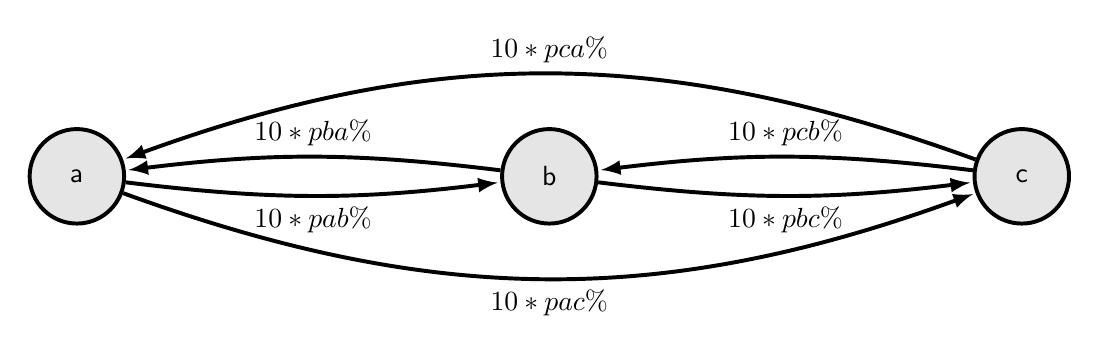
\begin{tikzpicture}[font=\sffamily]
  
  % Setup the style for the states
  \tikzset{node style/.style={state, 
                              minimum width=1.2cm,
                              line width=0.5mm,
                              fill=gray!20!white}}

  % Draw the states
  \node[node style] at (0, 0)     (a)     {a};
  \node[node style] at (6, 0)     (b)     {b};
  \node[node style] at (12, 0)    (c)     {c};

  % Connect the states with arrows
  \draw[every loop,
        auto=right,
        line width=0.5mm,
        >=latex]
      (a) edge[bend right=20, auto=right]  node {$\py{10*pac}\%$} (c)
      (a) edge[bend right=7, auto=right]   node {$\py{10*pab}\%$} (b)
      (b) edge[bend right=7, auto=right]   node {$\py{10*pba}\%$} (a)
      (b) edge[bend right=7, auto=right]   node {$\py{10*pbc}\%$} (c)
      (c) edge[bend right= 7, auto=right]  node {$\py{10*pcb}\%$} (b)
      (c) edge[bend right=20, auto=right]  node {$\py{10*pca}\%$} (a);
\end{tikzpicture}

Supponiamo che il rospo sia in {\sf a} al tempo $t=1$ 

\begin{itemize}
\item[1.] Qual è la probabilità che al tempo $t=2$ il rospo passi a {\sf c}~?

\item[3.] Qual è la probabilità che al tempo $t=3$ il rospo si trovi in {\sf c}~?

\end{itemize}

Esprimere il risultato come rapporto di numeri interi.

\begin{answer}

Siano $R_t$ le variabili aleatorie che danno la posizione del rospo al tempo $t$.

Dal diagramma inferiamo 

$\Pr(R_{2}={\sf c}~|~R_1={\sf a})\ =\kern1.2ex${\color{blue}$\py{pac/10}$\hfill Risposta 1}


Ci sono tre casi mutualmente escusivi per il percorso del rospo ai tempi $1,2,3$ 
che elenchiamo con le rispettive probabilità.

{\sf a,\ b,\ c}\hfill$\pyl{pab/10}\cdot\pyl{pbc/10} = \pyl{(pab * pbc) / 100}$

{\sf a,\ a,\ c}\hfill$\pyl{(10-pac-pab)/10}\cdot\pyl{pac/10} = \pyl{((10-pac-pab) * pac)/100}$

{\sf a,\ c,\ c}\hfill$\pyl{pac/10}\cdot\pyl{(10-pca-pcb)/10} = \pyl{(pac * (10-pca-pcb))/100}$


$\pyl{(pab * pbc) / 100} + \pyl{((10-pac-pab) * pac)/100} +  \pyl{(pac * (10-pca-pcb))/100} 
\ =\ $
{\color{blue}$\pyl{ (pab * pbc) / 100 + ((10-pac-pab) * pac)/100 +  (pac * (10-pca-pcb))/100}$\hfill Risposta 2}

\end{answer}
\end{xquestion}
  
  



\end{document}

